% !TeX root = ../main.tex
% Add the above to each chapter to make compiling the PDF easier in some editors.


\chapter{Functional B-Trees in Isabelle}\label{chapter:abs-set}

Proving higher level properties of data structures
tends to be easier on a functional level than on the imperative
level.
This is mostly due to the fact that many details of implementation
can be abstracted away or expressed in a simpler manner.
The work therefore begins with a functional specification of B-Trees
that is not aware of the existence of heaps or non-persistence.

\section{Basic Definitions}
\label{sec:basic-defs}
%Definition used for this implementation.
%(esp. order)
%note that k refers to keys+subtrees rather than only keys/subtrees (false! we have k pairs)

% TODO all function equations similar to math equations, setting variables in italics

As discussed in \Cref{chapter:introduction},
we define B-Trees recursively to either hold a list
subtrees and keys or be a completely empty Leaf.
The only room for interpretation is how to actually
store the subtrees and separators.
For Trees of variable but bounded size,
an explicit constructor may be given as for the 234-Trees in \parencite{DBLP:conf/itp/Nipkow16}.
However since the number of elements in B-Trees
is technically unbounded (as $k$ is not bounded)
we need to use an intermediate data structure,
a list, to store them.

In \parencite{DBLP:conf/popl/MalechaMSW10},
the B-Tree datatype was defined directly on the heap
and comprised a field that stored the height as well
as an array of fixed size that contains $key \times subtree$ pairs.
Since the list of children is exactly one longer than the list of keys,
a pointer to the last tree is added to the node in a special position.
By storing subtrees and keys next to each other,
definitions that relate subtrees to their immediately
neighboring separating keys (i.e. sortedness) becomes easier to define recursively.
This also implicitly enforces the relationship of the number of subtrees
and separators and makes the explicit use of length and index relationships unnecessary.
Therefore we chose to define B-Trees in a similar manner.

We will store subtrees and keys in pairs,
however with a different in-pair order,
such that the left subtree of a key is the left element
in a tuple and the key is the right element.
Moreover in a functional context, we will not make use of arrays
but rather resort to lists.
Other than in the imperative setting,
the explicit storing of the height inside a node is also
not required.
In \parencite{DBLP:conf/popl/MalechaMSW10} the height was
used to inductively define a shape predicate that is only valid
if the height decreases for subtrees.
However, the finite size of the abstract tree is an implicit
result of its recursive definition.
The definition follows and a visualization may be seen in \Cref{fig:btree-basic}.

\begin{lstlisting}[mathescape=true, language=Isabelle,label=lst:btree-def]
datatype 'a btree = Leaf | Node (( 'a btree * 'a ) list) ('a btree)
\end{lstlisting}

\begin{figure}
    \centering
    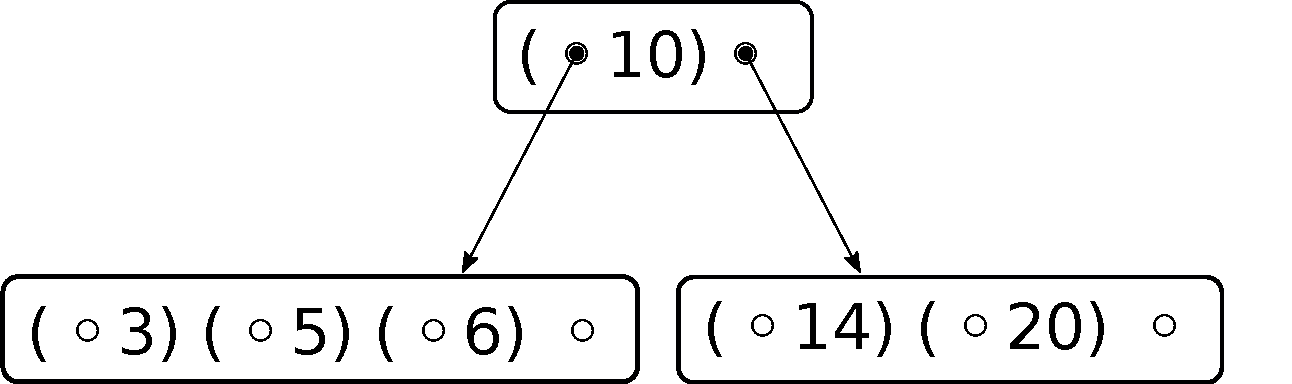
\includegraphics[width=0.5\linewidth]{figures/btree-basic.pdf}
    \caption{The B-Tree from figure \Cref{fig:btree-basic-nopair}.
    Subtrees and separators that lie in pairs in the implementation are surrounded by brackets.}
    \label{fig:btree-basic}
\end{figure}


The construction leads to the fact that it is easiest to relate any separator
to the subtree on the left, as this subtree is in the same tuple.
If a subtree on the right is required we may either match the
list to the right with the list constructor or 
choose the last tree.

The balancedness of a B-Tree is defined recursively, making use
of an intuitively defined height.\footnote{
    Note that the actual implementation of height is slightly different,
    however this is of no importance in any proofs but rather notationally convenient.
    Moreover, $`$ denotes the image all elements of a set for a given function.
}
There is a choice regarding how to obtain
the number to which the height of all subtrees has to be equal.
Either we fix the balancedness of a tree
on some existentially quantified number or to a known value.
Since we know the last tree in the node exists and further
know that if all subtrees of the node have the same height,
then their height is equal to the last tree,
we simply choose the height of the last tree as an anchor point.

\begin{lstlisting}[mathescape=true, language=Isabelle]

fun height :: 'a btree $\Rightarrow$ nat where
  height Leaf = 0 |
  height (Node ts t) = 1 + Max (height ` (set (subtrees ts@[t]))

fun bal :: 'a btree $\Rightarrow$ bool where
    bal Leaf = True |
    bal (Node ts t) = (
      ($\forall$sub $\in$ set (subtrees ts). height t = height sub) $\wedge$
      ($\forall$sub $\in$ set (subtrees ts). bal sub) $\wedge$
      bal t
    )
\end{lstlisting}

Further the order of the trees needs to be formally defined.
As discussed in \Cref{sec:data_structure_defs}, the most useful choice here is
to allow for at least $k$ and at most $2k+1$ subtrees.
Since the last subtree is fixed, and subtrees and children are residing as pairs in the same list,
we simply require the length of that list to be between $k$ and $2k$.
Note that we also need a special property $order^r$ for the root of the tree,
which has between one and $2k$ elements.
In mathematical equations, we will denote "order $k$ $t$" as "$\order_k t$"
for convenience (likewise for "order$^r$ $k$ $t$"), which is to be read as
"Tree $t$ is of order $k$".

\begin{lstlisting}[mathescape=true, language=Isabelle]

fun order :: nat $\Rightarrow$ 'a btree $\Rightarrow$ bool where
    order k Leaf = True |
    order k (Node ts t) = (
    (length ts $\ge$ k)  $\wedge$
    (length ts $\le$ 2*k) $\wedge$
    ($\forall$sub $\in$ set (subtrees ts). order k sub) $\wedge$
    order k t
  )

fun order$^r$ where
  order$^r$ k Leaf = True |
  order$^r$ k (Node ts t) = (
  (length ts $>$ 0) $\wedge$
  (length ts $\le$ 2*k) $\wedge$
  ($\forall$s $\in$ set (subtrees ts). order k s) $\wedge$
   order k t
)

\end{lstlisting}

We define the sortedness of a B-Tree based on the \textit{inorder} of the tree,
which is the concatenation of all elements of the tree in in-order traversal.
The concatenation function $concat$ on lists of strings
is employed to express the resulting string.
Note that this definition reads a bit inconveniently
as the node internal list is first mapped and then concatenated.
However since we make recursive use of the inorder-function
inside the mapping expression, we can only later cover up this expression
by using abbreviations.
In mathematical terms in the following, we will not distinguish between lists, 
pairs or trees when talking about their inorder representation.
The matching function from the below listing is meant instead.

\begin{lstlisting}[mathescape=true, language=Isabelle]
fun inorder :: 'a btree $\Rightarrow$ 'a list where
    inorder Leaf = [] |
    inorder (Node ts t) = 
        concat (map ($\lambda$ (sub, sep). inorder sub @ [sep]) ts)
        @ inorder t

abbreviation inorder_pair  $\equiv$ $\lambda$(sub,sep). inorder sub @ [sep]
abbreviation inorder_list ts $\equiv$ concat (map inorder_pair ts)
\end{lstlisting}

That way we can express sortedness of the tree $t$ as a simple $\sorted (\inorder t)$,
where $sorted$ is the property of being sorted strictly (with resprect to $<$)
in ascending order.
This definition is very compact and brings for another benefit
pointed out by Nipkow et al in \parencite{DBLP:conf/itp/Nipkow16}.
Many properties of search trees follow intuitively by considering
the inorder view on the tree.
Usually, it invariant for all operations (i.e. stealing from the right neighbor node)
or only deviates in a manner we expect it to deviate given the inorder view
(i.e. insert an element at the correct position).
We will see later how the use of this fact comes in handy for proving
important properties of the implementation.

Since our B-Tree definition really only makes sense for positive $k$,
we obtain the following overall invariant for B-Trees.

\begin{definition}
    $k > 0 \Longrightarrow \btree_k t := \bal t \wedge \order^r_k t \wedge \sorted (\inorder t)$
\end{definition}

All trees that satisfy this invariant have a very small
height considering the number of inserted elements.
This fact is examined closer in the following section.
 % TODO note benefit over btree_sorted

\section{Height of B-Trees}

%Height etc.
As pointed out by Bayer in the first paper describing B-Trees,
the height of B-Trees is logarithmic with respect to the number
of nodes of the tree. \parencite{DBLP:journals/acta/BayerM72}
The paper even gives a precise lower and upper bound,
which will be quickly sketched in the following.

First, we define the number of nodes in a tree:
\begin{lstlisting}[mathescape=true, language=Isabelle]
fun nodes :: 'a btree $\Rightarrow$ nat where
    nodes Leaf = 0 |
    nodes (Node ts t) =
        1 + $\sum$t$\leftarrow$subtrees ts. nodes t + nodes t
\end{lstlisting}

%To work with this equation, we just need to add one auxiliary lemmas to the standard canon
%\begin{lemma}
%\begin{lstlisting}[mathescape=true, language=Isabelle]
%    sum_list (replicate n c) = n*c
%\end{lstlisting}
%\end{lemma}

We obtain bounds
on the number of nodes of an subtree with respect to its height
by induction on the computation of the nodes function.

\begin{lemma}
    \label{lem:bound_internal_node}
    $\order_k t \wedge \bal t \longrightarrow$
    \begin{align}
        (k+1)^{\height t} - 1 &\le \nodes t * k \\
        \nodes t * 2k &\le (2k+1)^{\height t} - 1
    \end{align}
\end{lemma}

From \Cref{lem:bound_internal_node} we can almost directly obtain
the bounds on valid roots of B-Trees.
The only difference to the bound of internal nodes occurs on the lower bound side.
The issue here is that a root node may contain less elements than
a valid internal node (namely only one), which yields two subtrees with known height
plus one for the node itself.
Note that these are the exact bounds obtained by Bayer et al. in \parencite{DBLP:journals/acta/BayerM72},
except for the fact that we have generalized the equation,
incorporating whether $t$ is a tree or not.\footnote{
    If $t$ is in fact a Leaf,
    $2((k+1)^{\height t - 1} - 1) \div k + (t \neq Leaf)$ becomes a fancy way of writing $0$.
}

\begin{theorem}
    $\rootorder_k t \wedge \bal t \wedge k > 0 \longrightarrow$
    \begin{equation}
        2((k+1)^{\height t - 1} - 1) \div k + (t \neq Leaf) \le \nodes t \le ((2k+1)^{\height t} - 1) \div 2k
    \end{equation}
\end{theorem}

These results are very interesting, because
the runtime of all further operations will more or less trivially be
directly proportional to the height of the tree.
Therefore, we are glad to see that the height is logarithmic
with respect to the number of nodes stored in the tree.

These bounds are sharp.
We prove this by providing 
functions that generate exactly those trees
that satisfy the requirements of B-Trees, have a given height
and satisfy the inequality with equality in \Cref{lst:sharp-trees-def}.
As might be expected, these trees are simply those trees
that are minimally or maximally filled in each node with respect
to the order property.

%TODO (?) images of slim/full trees
\begin{figure}
\begin{lstlisting}[mathescape=true, language=Isabelle,label={lst:sharp-trees-def},
    caption={The functions generating trees with minimal size and maximal size for given height.}]

fun full_node where
  full_node k c 0 = Leaf |
  full_node k c (Suc n) = (
      Node
        (replicate (2*k) ((full_node k c n),c))
        (full_node k c n)
  )

fun slim_node where
  slim_node k c 0 = Leaf |
  slim_node k c (Suc n) = (
      Node
        (replicate k ((slim_node k c n),c))
        (slim_node k c n)
    )

definition full_tree = full_node

fun slim_tree where
  slim_tree k c 0 = Leaf |
  slim_tree k c (Suc h) =
    Node
        [(slim_node k c h, c)]
        (slim_node k c h)

\end{lstlisting}
\end{figure}

The proof for internal nodes follows by induction over the creation.

\begin{lemma} $t_f := \fullnode k\ a\ h \wedge t_s := \slimnode k\ a\ h \longrightarrow$
    \begin{align}
    h = \height t_s = \height t_f \wedge \\
    ((2k+1)^h - 1) &= \nodes t_f * (2k) &\wedge \order_k t_f \wedge \bal t_f \\ 
    ((k+1)^h - 1) &= \nodes t_s * k  &\wedge \order_k t_s \wedge \bal t_s
    \end{align}
\end{lemma}

The rule for the roots follows directly, making use of the lemma
for the internal nodes.
Note how for the root node the results is simply two times the
value for trees of one height less, which are the minimally
required two subtrees.

% TODO prove div version of thm
\begin{theorem}
    $k > 0 \wedge t_f := \fulltree k\ a\ h \wedge t_s := \slimtree k\ a\ h \longrightarrow$
    \begin{align*}
    h = \height t_s &= \height t_f &\wedge \\
        ((2k+1)^h - 1) \div 2k &= \nodes t_f &\wedge \rootorder_k t_f \wedge \bal t_f \\ 
        2((k+1)^h - 1) \div k + (t_s \neq Leaf) &= \nodes t_s &\wedge \rootorder_k t_s \wedge \bal t_s
    \end{align*}
\end{theorem}


\section{Set operations}

With the definition of B-Trees come a number of operations that allow
for set-like operations on the trees -
queries whether an element is contained, insertion and deletion.
In the Isabelle/HOL framework, there is a standard interface
for data structures that provide an implementation of sets.

\subsection{The Set Interface}
% Description of the set interface

An implementation \textit{'a t} of the sets of elements of type \textit{'a} is required to provide the following
operations

\begin{itemize}
    \itshape
    \item empty :: 'a t
    \item isin :: 'a t $\Rightarrow$ 'a $\Rightarrow$ bool
    \item insert :: 'a $\Rightarrow$ 'a t $\Rightarrow$ 'a t
    \item delete :: 'a $\Rightarrow$ 'a t $\Rightarrow$ 'a t
\end{itemize}

Additionally, an invariant \textit{invar :: 'a t $\Rightarrow$ bool} has to be supplied.
For this work, using the definition from \Cref{lst:btree-def},
we consider \textit{'a t = 'a btree}.
The standard approach is to provide functions on B-Tree and show
that they have the same effect as membership test, insertion and deletion 
in abstract sets with the same elements
(i.e. $invar\ t \Longrightarrow set\ (insert\ x\ t) = set\ t \cup {x}$ ).
Further, the invariant needs to remain valid for the results of the operations
as well as the $empty$ element (i.e. $invar\ t \Longrightarrow invar\ (insert\ x\ t)$).
In order to obtain such a set, an additional \textit{abstraction function}
has to be provided, \textit{set :: 'a t $\Rightarrow$ 'a set}.

We know from \Cref{sec:basic-defs} that one of the invariants
of the tree is that it is always sorted.
While this is expressed in a somewhat cumbersome manner
in the original definition by Bayer \parencite{DBLP:journals/acta/BayerM72},
this requirement is nothing else but a sortedness of the inorder view of the tree.
Knowing this, we resort to a specialized Set interface
proposed by Nipkow \parencite{DBLP:conf/itp/Nipkow16}.
Their approach yielded automatic proofs for 2-3-Trees
and 2-3-4-Trees, which are specializations of B-Trees.
The modified Set interface reasons based on the inorder
view on the tree instead of the \textit{set} abstraction.

The invariant and inorder functions for this set interface
follow directly from the definition of B-Trees.
Hence, we specify $k > 0 \wedge \order^r_k t \wedge \bal t$
as the invariant of B-Trees and use
the concatentation function from \Cref{sec:basic-defs} to specify the
inorder abstraction \textit{inorder :: 'a t $\Rightarrow$ 'a list}.
The interface is then implemented by providing set operations
and the proofs of invariant preservation.

Some parts of the Set specification are trivial.
In the following, \textit{Leaf} is an empty tree and hence represents
the empty set, satisfying the first part of the specification.
It can be seen directly that the leafs already satisfy all three properties.
The following sections will describe the implementation of the
non-trivial set operations.

\subsection{The split-Function}
% Description of the implementation of the set interface.

Naturally the set operations are defined recursively on the nodes of the tree.
Since each node contains a non-trivial number of elements,
a function to navigate to the correct separator and subtree is central to all operations.

We call this function \textit{split}-function,
determining the position in the list of separators and subtrees.
At the "correct" position, the range spanned by the left subtree
and the separator is exactly the range in which the desired element
must be contained if it is contained in the tree.
At this position, either the separator is equal to the desired value or
we need to recurse into the left subtree.
This approach is similar to the one found in the work of Malecha and Fielding \parencite{DBLP:conf/popl/MalechaMSW10,Fielding80}.\footnote{
    In Fieldings approach the corresponding function is called \textit{index}.
    Malecha calls it \textit{findSubtree}.
}
Usually however, it is integrated into the set-operation
by a linear search that is promised to be replaced by a more efficient binary search
in the actual implementation \parencite{DBLP:books/daglib/0023376,DBLP:journals/acta/BayerM72}
or left in the final code \parencite{DBLP:journals/sosym/ErnstSR15}

The precise inner workings of the split function are not of interest here
and actually are not supposed to be interesting on the functional level.
Of course \textit{some} kind of function is required that correctly splits
the key-value list and an example is given in \Cref{fig:linear_split}.
In the process of implementing the set specifications,
this concrete function was used to explore the provability of the set methods.
However it quickly turned out that 1) only specific lemmas about the split
function are useful during proofs and 2) only relying on an abstract specification of
the split method would simplify integrating alternative splitting functions.
Most notably, the abstraction allows to later plug in a very efficient splitting
function, e.g. based on binary search.

\begin{figure}
    
\begin{lstlisting}[mathescape=true, language=Isabelle]
fun linear_split_help where
  linear_split_help [] x prev = (prev, []) |
  linear_split_help ((sub, sep)#xs) x prev = (
      if sep < x then
        linear_split_help xs x (prev @ [(sub, sep)])
      else
        (prev, (sub,sep)#xs)
  )

fun linear_split:: ('a btree$\times$'a) list $\Rightarrow$ 'a $\Rightarrow$ (_ list $\times$ _ list) where
  linear_split xs x = linear_split_help xs x []
\end{lstlisting}
\caption{A function implementing the split function specifications.
It scans linearly through the list, returning the first tuple where the separator
or subtree could potentially contain the value $x$}
\label{fig:linear_split}

\end{figure}

Therefore all set functions are defined based the following requirements:

\begin{itemize}
    \item $\splitfun xs\ p = (ls,rs) \Longrightarrow xs = ls @ rs$
    \item $\splitfun xs\ p = (ls@[(sub,sep)],rs) \wedge \sorted (\separators xs) \Longrightarrow sep < p$
    \item $\splitfun xs\ p = (ls,(sub,sep)\#rs) \wedge \sorted (\separators xs) \Longrightarrow p \le sep$
\end{itemize}

Described in natural language, the split function should return two sublists
that concatenate to the original list.
Further if the elements came in sorted order,
the list is split such that the key to the left is strictly less than the desired value
and the key to the right should be less or equal.

Note how the split function really only needs to
consider the separators and not the subtrees themselves.
By requiring only sortedness of the separators,
we simplify the proofs of showing that a certain function
fulfils the split abstraction.
If the whole tree is sorted, the separators are sorted too.
We prove this once and from it follows that
we may use the split function for sorted trees as well.

The abstraction was formulated in a locale.
Inside the locale we have access to exactly the specified split function,
without knowing anything about the composition of that function.

\subsection{Membership tests}

%-------------------------------------------------
% TODO move to abstract description?
The simplest operation required in the Set interface is
the \textit{isin} function.
It is required to operate on the B-Tree 
the same way as membership queries on the set abstraction.
% Note reference to i.e. Bauer retrieval algorithm
The definition in \Cref{lst:isin-fun} also shows exemplary usage of the split function.
In case the right part of the split list is non-empty,
we check the element at that level or recurse in the given subtree.
Otherwise, we may directly recurse to the last tree in the node.\footnote{
    Since this function recurses on the split function,
    in order to show that this function terminates, we need to tell
    the system that the obtained subtrees are of smaller size than the current tree.
    Adding this fact to the default termination simplification set resolves
    the issue for all coming functions.
}
%-------------------------------------------------

\begin{figure}
\begin{lstlisting}[mathescape=true, language=Isabelle, caption=The \textit{isin} function, label=lst:isin-fun]
fun isin:: 'a btree $\Rightarrow$ 'a $\Rightarrow$ bool where
    isin (Leaf) y = False |
    isin (Node ts t) y = (
        case split ts y of (_,(sub,sep)#rs) $\Rightarrow$ (
            if y = sep then
                True
            else
                isin sub y
        )
    | (_,[]) $\Rightarrow$ isin t y
    )
\end{lstlisting}
\end{figure}

By the standard set interface the operation is only required to work on
sorted, balanced trees of a certain order, however only the first property
is actually required for correctness.
The following lemma shows the required property of the function

\begin{theorem}
    \label{thm:isin-set}
    $\sorted (\inorder t) \Longrightarrow \isinfun t\ x = (x \in \setfun (\inorder t))$
\end{theorem}

It follows by induction on the evaluation of the isin function.
To prove it, we invoke two specialized lemmas,
that simplify arguments about the choice of the node for recursion.
The kind of lemmas are of special interest as they specialize
an idea proposed in \parencite{DBLP:conf/itp/Nipkow16} and similar lemmas
are used for the correctness proofs of insert and delete alike.

\begin{lemma} $\sorted (\inorder (Node\ ts\ t) \wedge \splitfun ts\ x = (ls, rs) \Longrightarrow$ \\
    \begin{center}
    $x \in (\setfun (\inorder (Node\ ts\ t))) = (x \in \setfun (\inorder rs @ \inorder t))$
    \end{center}
\end{lemma}

The idea of this fact is to argue that, if the split function has provided
us with a given splitting, it is safe to limit the further search
to the right side of the split.
It follows directly from the requirements on the split function.
If $rs$ is empty, we can follow that the element has to reside in the inorder
of the last tree of the node.
When used in the inductive proof of \Cref{thm:isin-set}, we can then deduce that this is
equal to \textit{isin t x}, the branch taken in the isin-function
(see \Cref{lst:isin-fun}) for an empty right split result.
If $rs$ is not empty, we need an additional lemma.

\begin{lemma}
    $\sorted (\inorder (Node\ ts\ t)) \wedge \splitfun ts\ x = (ls, (sub,sep)\#rs) \wedge sep \neq x \Longrightarrow$ \\
    \begin{center}
    $x \in (\setfun (\inorder ((sub,sep)\#rs) @ \inorder t)) = (x \in \setfun (\inorder sub))$
    \end{center}
\end{lemma}

With this lemma we know that the first subtree on the right part of the split
is the correct child to recurse into.
The requirement of $sep \neq x$ is because if $sep = x$,
no recursion is required at all.
The desired element was just found.

This operation has no effect on the tree, it only walks through it.
This fact follows directly due to the persistence of functional data structures.
Hence, no proof of invariant preservation is required,
in contrast to the following tree-modifying operations.

\subsection{Insertion}
\label{sec:abs-ins}


% TODO what is this for?
%There are not many provably correct functional implementations to our knowledge.
%However there is a relationship between 234-Trees and B-Trees,
%due to which the approach to the functional definition is inspired by the implementation
%in \parencite{DBLP:conf/itp/Nipkow16}.
%In that work, a correct implementation of the Set interface for 234-Trees 
%are provided.

The implementation of the insertion function
as described in \Cref{par:intro-ins} is documented in \Cref{lst:ins-fun}.
However, rather than manually checking whether the lowest level was reached,
we recurse until we reach a Leaf node.
Inserting into it will lead to an overflow that can be handled
by the lowest internal nodes in the same manner as for other internal nodes.

To modularize insertion, the check for the overflow of a nodes list has been
extracted to the function $node_i$.
It returns data in a new datatype called $up_i$, which
carries either a singleton valid B-Tree or two trees and a separator
that could correctly be part of a node when placed next to each other.
This construction is useful for handling overflow
in a functional context and appears similarly in \parencite{DBLP:conf/itp/Nipkow16}.

The $ins$ function is a recursive helper function,
that recurses down into the correct leaf node for inserting the desired element.
The recursive call may have caused an overflow in a lower node.
If an overflow occured, an additional element and
new subtree is inserted into the
current nodes list with the help of \textit{node}$_i$,
the result of which is again of type $up_i$ to indicate to
the parent whether overflow occurred.
If no overflow occured we may directly return $T_i$ of the current node
to indicate no overflow.

Finally, the \textit{insert} function calls the \textit{ins} helper function
and transforms the result into a valid B-Tree.

\begin{figure}
    
\begin{lstlisting}[mathescape=true, language=Isabelle, label=lst:ins-fun, caption={
    The \textit{insert} function
}]
datatype 'b up$_i$ = T$_i$ 'b btree | Up$_i$ 'b btree 'b 'b btree

fun split_half where
  split_half xs = (take (length xs div 2) xs, drop (length xs div 2) xs)

fun node$_i$ :: nat $\Rightarrow$ ('a btree $\times$ 'a) list $\Rightarrow$ 'a btree $\Rightarrow$ 'a up$_i$ where
  node$_i$ k ts t = (
  if length ts $\le$ 2*k then T$_i$ (Node ts t)
  else (
    case split_half ts of (ls, (sub,sep)#rs) $\Rightarrow$
      Up$_i$ (Node ls sub) sep (Node rs t)
    )
  )

fun ins :: nat $\Rightarrow$ 'a $\Rightarrow$ 'a btree $\Rightarrow$ 'a up$_i$ where
  ins k x Leaf = (Up$_i$ Leaf x Leaf) |
  ins k x (Node ts t) = (
  case split ts x of
    (ls,(sub,sep)#rs) $\Rightarrow$ 
      (if sep = x then T$_i$ (Node ts t)
      else
        (case ins k x sub of 
          Up$_i$ l a r $\Rightarrow$
            node$_i$ k (ls @ (l,a)#(r,sep)#rs) t | 
          T$_i$ a $\Rightarrow$ T$_i$ (Node (ls @ (a,sep) # rs) t))) |
    (ls, []) $\Rightarrow$
      (case ins k x t of
         Up$_i$ l a r $\Rightarrow$
            node$_i$ k (ls@[(l,a)]) r |
         T$_i$ a $\Rightarrow$ T$_i$ (Node ls a)
  )
)

fun tree$_i$ :: 'a up$_i$ $\Rightarrow$ 'a btree where
  tree$_i$ (T$_i$ sub) = sub |
  tree$_i$ (Up$_i$ l a r) = (Node [(l,a)] r)

fun insert::nat $\Rightarrow$ 'a $\Rightarrow$ 'a btree $\Rightarrow$ 'a btree where
  insert k x t = tree$_i$ (ins k x t)
\end{lstlisting}

\end{figure}

\begin{figure}
    \centering
    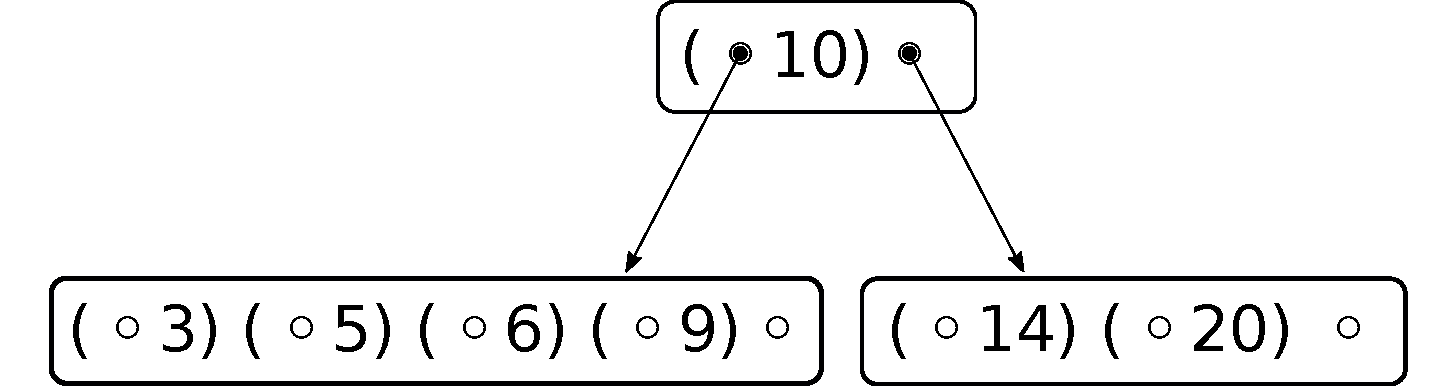
\includegraphics[width=0.48\linewidth]{figures/btree-basic-ins9.pdf}\\
    \vspace*{1cm}
    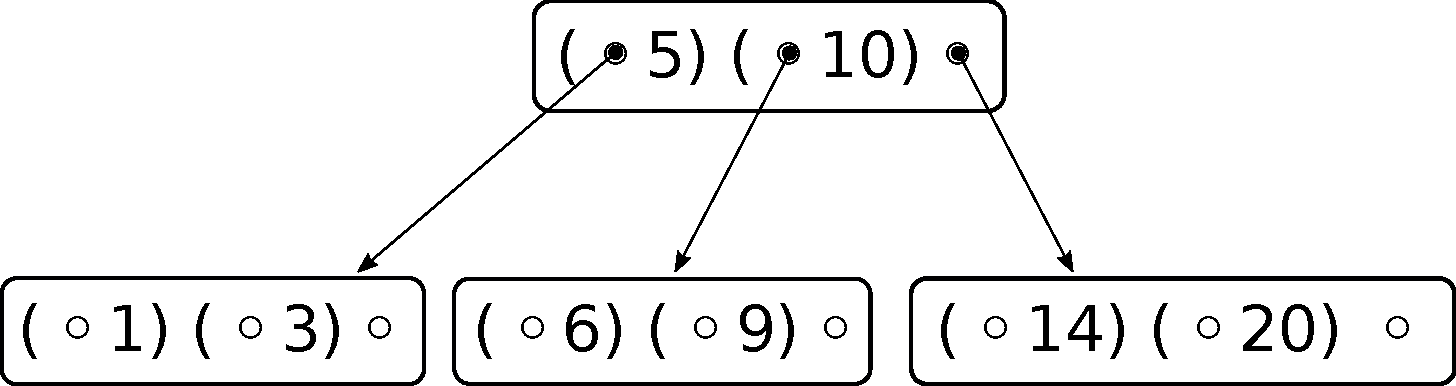
\includegraphics[width=0.48\linewidth]{figures/btree-basic-ins9-ins1.pdf}
    \caption{The tree from \Cref{fig:btree-basic} after 
    successive insertion of $9$ (top) and $1$ (bottom).}
    \label{fig:btree-basic-ins}
\end{figure}
%TODO

To fulfil the Set interface requirements,
we need to show that this function preserves the invariants
and acts the same as inserting element $x$ into the inorder list of the tree.

Note that for the above proofs, a separate notion of height, balancedness and order
was introduced for the $up_i$ datatype.
Height and balancedness are
defined such that the property is invariant to splitting and merging of nodes.
For example, "$\height ts\ t = \heightup_i (\node_i k\ ts\ t)$".
Note that this is not the same as applying the original functions
to the tree obtained by tree$_i$.
Order of up$_i$ elements however simply subsumes that all subtrees have
the given order.
Naturally, making a one-element tree of an up$_i$ element will thus
give a node of root-order, while inserting the elements
will not violate the recursive order requirement.

Proving the balancedness invariant requires as additional lemma that
the height is invariant under insertion.
Technically, height preservation is only required when modifying balanced
trees, however we have shown the stronger statement that this is even the case for non-balanced trees.
This follows by induction using the
associativity and commutativity of the maximum function
and with it the proof for balancedness follows much the same way.
Overall, the fact that the operation does preserve balancedness and
height should come at no surprise.
After all, the operations are never directly affecting the height of any tree,
and the all trees generated by splitting a node comprise trees
that had been there before, now simply distributed along to node
in the same level.

\begin{lemma}
    \begin{align*}
    \height t & = \height (\insfun_k x\ t) \\
    \bal t & \Longrightarrow \bal (\insfun_k x\ t)
    \end{align*}
\end{lemma}

Now for the proof of preserving the order invariant.
Since the central function to ensure order is the node$_i$ function,
we first show the following lemma:

\begin{lemma}
\label{lem:nodei-order}
    If all children have order $k$ and $\length ts \ge k$ and $\length ts \le 4k+1$
    then all trees in $\node_i k\ ts\ t$ have order $k$.
\end{lemma}

Even though in the case of insertion the length of the list
never exceeds $2k+1$, the statement holds up to $4k+1$.
The statement is proven by case distinction whether "$\length ts \le 2k$".
Looking at the definition in \Cref{lst:ins-fun}
we see that if this is the case nothing happens and the lemma is trivial.
In case "$\length ts > 2k$", a split occurs.
The median element is passed up as a seperator, leaving
$\lfloor\frac{\length ts}{2}\rfloor$ and $\lceil\frac{\length ts}{2}\rceil - 1$
elements for the left and right node respectively.
Given the constraint on the maximum length of $ts$
this will always be below or equal $2k$.
Further, as we require a size of at least $2k+1$ elements for a split to occur,
the resulting nodes each have at least $k$ elements.
The argument hardly changes comparing the upper bounds $2k+1$ and $4k+1$,
but with the former upper bound it can be used for merging nodes
in the deletion function as well.

Using the above, the order invariant for \textit{ins}
follows quite directly by induction.

\begin{lemma}
    $\order_k t \Longrightarrow \order_k (\insfun_k x\ t)$
\end{lemma}

Since the invariant on B-Trees only requires a root order of $k$ on the
root, we additionally derive versions of the invariants
for root order.
They are straightforward however as all trees in the inductive case
have order $k$, for which preservation was already proven.
Putting things together, we obtain preservation of the invariants.

\begin{theorem}
    $\order^r_k t \wedge \bal t \Longrightarrow
    \order^r_k (\insertfun_k x\ t) \wedge \bal (\insertfun_k x t)$
\end{theorem}


The set interface further requires that the insertion returns a tree
that has the same inorder view as the original inorder with the element
inserted at the correct position.

Looking at the \textit{ins} function in \Cref{lst:ins-fun},
we see that in an inductive proof the main obligation
is to argue for the choice of the subtree in case of recursion.
Similar to the proof of \Cref{thm:isin-set},
we use two auxiliary lemmas, that turn the remaining
proof in simple case distinctions and chains of equations.

\begin{lemma}
    $\sorted(\inorder (Node\ ts\ t)) \wedge \splitfun ts\ x = (ls, rs) \Longrightarrow$ \\
    \begin{center}
    $\inslist x\ (\inorder (Node\ ts\ t))) = \inorder ls\ @\ \inslist x\ (\inorder rs\ @\ \inorder t)$
    \end{center}
\end{lemma}

\begin{lemma}
    $\sorted (\inorder (Node\ ts\ t)) \wedge \splitfun ts\ x = (ls, (sub,sep)\#rs) \wedge sep \neq x \Longrightarrow$ \\
    \begin{center}
    $\inslist x\ (\inorder ((sub,sep)\#rs)\ @\ \inorder t)) =$\\
    $ (\inslist x\ (\inorder sub))\ @\ sep \# \inorder rs\ @\ \inorder t$
    \end{center}
\end{lemma}

The only case not covered by the above lemmas is the case $sep = x$.
In that case, the tree does not change.
This is due to the fact that $x$ is already in the set represented by the tree
and hence does not need to be inserted.
The same happens when inserting $x$ into a list that already contains $x$
(i.e. the inorder of the tree),
which follows simply by induction on the list.

\begin{lemma}
    $\sorted xs \wedge x \in \setfun xs \Longrightarrow \inslist x\ xs = xs$
\end{lemma}

The above lemmas are all we need to show correctness
of the \textit{ins} function inductively.
The theorem for \textit{insert} follows again automatically,
which concludes the proof of the insertion part.

\begin{theorem}
    \label{thm:ins-set}
    $\order_k t \wedge \bal t \wedge \sorted  (\inorder t)\Longrightarrow$\\
    \begin{center}
    $\inorder (\insertfun_k x\ t) = \insertfun_{list} x\ (\inorder t)$
    \end{center}
\end{theorem}


\subsection{Deletion}


\begin{figure}
\begin{lstlisting}[mathescape=true, language=Isabelle,label={lst:rebalance-def},
    caption={The rebalancing functions}]
fun rebalance_middle_tree where
  rebalance_middle_tree k ls Leaf sep rs Leaf = (Node (ls@(Leaf,sep)#rs) Leaf) |
  rebalance_middle_tree k ls (Node mts mt) sep rs (Node tts tt) = (
    if length mts $\ge$ k $\wedge$ length tts $\ge$ k then
        Node (ls@(Node mts mt,sep)#rs) (Node tts tt)
    else (
        case rs of [] $\Rightarrow$ (
            case node$_i$ k (mts@(mt,sep)#tts) tt of
                T$_i$ u $\Rightarrow$ Node ls u |
                Up$_i$ l a r $\Rightarrow$ Node (ls@[(l,a)]) r
            ) |
        (Node rts rt,rsep)#rs $\Rightarrow$ (
            case node$_i$ k (mts@(mt,sep)#rts) rt of
                T$_i$ u $\Rightarrow$
                   Node (ls@(u,rsep)#rs) (Node tts tt) |
                Up$_i$ l a r $\Rightarrow$
                   Node (ls@(l,a)#(r,rsep)#rs) (Node tts tt)
            )
        )
    )

fun rebalance_last_tree where
    rebalance_last_tree k ts t = (
        case last ts of (sub,sep) $\Rightarrow$
            rebalance_middle_tree k (butlast ts) sub sep [] t
    )
\end{lstlisting}
\end{figure}

The procedures described in \Cref{par:intro-del}
are implemented here with a
certain flavor due to the setup of B-Trees.
The $rebalancing$ as implemented in \Cref{lst:rebalance-def}
comprises merging and splitting neighboring nodes.
For simplicity of the function and proofs, we always
merge with the right sibling.
The only exception, which is unavoidable due to the asymmetry of the data structure,
is an underflow in the last subtree.
It will be merged with the second-to-last subtree, the last
tree in the variable length list of the node.
Note also how the tree does not change when asked to rebalance a leaf.
The reason is that rebalancing leafs may only happen if it is preceded
by deletion from a leaf - which does not change the tree at all.

The other detail is regarding the \textit{split\_max} function
defined in \Cref{lst:del-def}.
Here some freedom exists whether to swap with the maximum lesser
or the minimum greater element in the tree.
In our setup, the last tree of the node is explicitly stored in each node
and the left subtree of a separator lies within the same
pair inside the node list.
Using pattern matching, it is hence significantly
easier to obtain the maximum of the left subtree
than the minimum of the right subtree.
Therefore we will always swap with the former, maximal lesser element.
%---------------------------------------------------------

The most interesting property for the rebalancing operations is the order property,
which is meant to be restored after potential underflows.
It is important to note here that we cannot guarantee
that at least one element remains in the node that
is passed back upwards.
However we can guarantee that all subtrees of the result are of order $k$
and that there are no more than $2k$ elements in the result.
We say that if a tree $t$ has at most $2k$ elements
and all subtrees of $t$ have order $k$, then $t$ has
 \textit{almost order} of $k$, or $\order^a_k t$.

\begin{lemma}
    If all subtrees in ls, rs are of order k 
    and of sub and t, only one may have almost order k and the other has order k,
    and all subtrees have equal height, then \\
    \begin{center}
    $\order^a_k (\rebalancemt_k ls\ sub\ sep\ sep\ rs\ t)$
    \end{center}
\end{lemma}

It might be suprising that we require all subtrees to have equal height
for this operation.
However, a close look at \Cref{lst:rebalance-def} clarifies that
in order to successfully rebalance an internal node, we need neighboring
nodes that are not leafs.
As this fact is already expressed in the pattern matching of the function,
it is simply \textit{undefined} for unbalanced trees.
But we know that the B-Tree is always balanced, so we may assume it for all proofs
involving \textit{rebalance\_middle\_tree}.

For this proof, we re-use \Cref{lem:nodei-order},
as two nodes of order $k$ will always contain
a maximum of $4k+1$ separators.
The case that the subtree and separator list becomes zero
is exactly when a root with minimal size underflows.
After this operation the tree shrinks in height.
The shrinked tree then is exactly the one remaining subtree in the original node.
See the operation \textit{reduce\_root} in \Cref{lst:del-def} for the exact implementation
of this step.

\begin{figure}
\begin{lstlisting}[mathescape=true, language=Isabelle,label={lst:del-def},
    caption={The $delete$ function}]

fun split_max where
    split_max k (Node ts t) = (
        case t of Leaf $\Rightarrow$ (
            let (sub,sep) = last ts in (Node (butlast ts) sub, sep)
        ) |
        _ $\Rightarrow$ case split_max k t of (sub, sep) $\Rightarrow$
                (rebalance_last_tree k ts sub, sep)
        )

fun del where
    del k x Leaf = Leaf |
    del k x (Node ts t) = (
    case split ts x of (ls,[]) $\Rightarrow$
        rebalance_last_tree k ls (del k x t) |
    (ls,(sub,sep)#rs) $\Rightarrow$
        if sep $\neq$ x then
            rebalance_middle_tree k ls (del k x sub) sep rs t
        else if sub = Leaf then
            Node (ls@rs) t
        else let (sub_s, max_s) = split_max k sub in
            rebalance_middle_tree k ls sub_s max_s rs t
    )
 
fun reduce_root where
    reduce_root Leaf = Leaf |
    reduce_root (Node ts t) = (case ts of
        [] $\Rightarrow$ t |
        _ $\Rightarrow$ (Node ts t)
    )
 
fun delete where delete k x t = reduce_root (del k x t)
\end{lstlisting}
\end{figure}

\begin{figure}
    \centering
    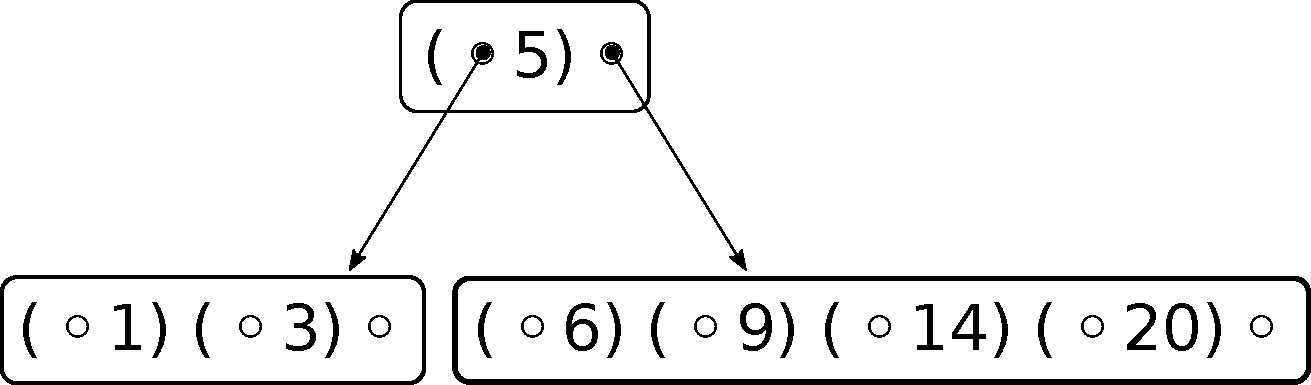
\includegraphics[width=0.48\linewidth]{figures/btree-basic-ins9-ins1-del10.pdf}\\
    \vspace*{1cm}
    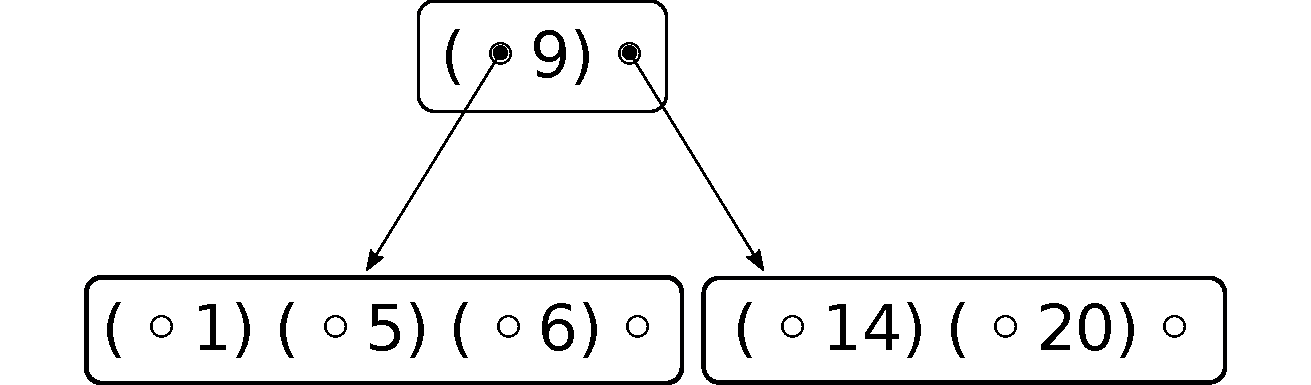
\includegraphics[width=0.48\linewidth]{figures/btree-basic-ins9-ins1-del10-del3.pdf}
    \caption{The tree from \Cref{fig:btree-basic-ins} after 
    successive deletion of $10$ (top) and $3$ (bottom).
    Note how the final result differs from approaches that would only steal single elements
    from neighbors to hanlde underflow.}
    \label{fig:btree-basic-del}
\end{figure}

From this fact follows further, that for the results of all intermediate functions
in the deletion process, $\order^a k$ of the results can be guaranteed.
Since the last subtree in the result of deletion has order $k$,
and for more than one subtree the node has root order,
the result of \textit{delete} always has at least $\order^r k$.

The proofs for balancedness invariance follow similarly to
the ones in \Cref{sec:abs-ins} by first showing height invariance.
The properties follow using the associativity
and commutativity of the maximum operation.
The proof of height, balancedness and order
are interleaved among the proofs for the
intermediate functions, especially
\textit{split\_max} and \textit{rebalance\_middle\_tree},
which are only well defined for balanced trees
and \textit{split\_max}, which requires at least
one element in the node list, an equivalent
to $\order^r k$.

With the basic functionalities covered,
the invariant preservation of the \textit{del} function
can be derived inductively.
Note that the function will return a tree of almost order $k$,
where the remaining root-underflow is coverered by \textit{reduce\_root}.
Moreover we do not need an additional lemma
for an input with nodes that have normal order $k$.
As $k > 0$, order $k$ implies a root order of $k$.
And even though that it might be beneficial to know
the input to have normal order, this is not the case.
Since the rebalancing functions do only require
almost order $k$ to return normally ordered trees,
the resulting list will always be sufficient.

\begin{lemma}
    $k > 0 \wedge \order^r_k t \wedge \bal t \Longrightarrow
    \order^a_k (\delfun_k x\ t) \wedge \bal (\deletefun_k x t)$
\end{lemma}

Putting together the proofs on balancedness and
order, we obtain the fact about the invariant
preservation of the deletion function that is required by the set interface.

\begin{theorem}
    $k > 0 \wedge \order^r_k t \wedge \bal t \Longrightarrow$ \\
    \begin{center}
    $\order^r_k (\deletefun_k x\ t) \wedge \bal (\deletefun_k x t)$
    \end{center}
\end{theorem}

Note that now (as opposed to insertion) $k > 0$ is required.
The main reason is that, while it was not too important for most of the proofs until now,
B-Trees do only work for positive $k$.
If $k = 0$, rebalancing would not always work anymore
as we could not be certain to have at least two subtrees per node.

In order to prove that \textit{delete} acts the same as
\textit{delete}$_{list}$ on the inorder of the tree,
we need to show some inorder properties for the intermediate functions.
For the \textit{del} helper function, 
we use the same specialized lemmas
as for \Cref{thm:isin-set} and \Cref{thm:ins-set}
and induct over the execution of the \textit{del}-function.
% TODO state or no state?

Rather than stating the specialized lemmas again at this point, we would like to point
out the elegance of the inorder method at this point.

The reason the rebalancing functions preserve the sortedness and set properties
is plain when considering the inorder view of the tree:
it does not change at all.
A manual proof about the set and sortedness properties
would require complicated, unnecessarily lengthy proofs.
For the inorder view, 
since the results can be easily simplified, even without recursive calls,
the property follows automatically.

\begin{lemma}
    \label{lem:rebalance-inorder}
    All subtrees have the same height $\Longrightarrow$ \\
    \begin{equation*}
    \inorder (\rebalancemt_k ls\ sub\ sep\ rs\ t) =\\
    \inorder (Node (ls@(sub,sep)\#rs)\ t)
    \end{equation*}
\end{lemma}

Considering the function split\_max,
the standard approach would require showing
tideously that the element returned is in fact the maximum of the whole tree
and showing that the remaining tree union the maximum element
gives the whole original tree set.
Instead we simply show the following,
comprising both facts:

\begin{lemma}
    \label{lem:splitmax-inorder}
    If t has more than two subtrees, and the last two are equally high, then
    \begin{equation*}
    \inorder (\splitmax_k t) = \inorder t
    \end{equation*}
\end{lemma}

This fact follows easily by induction on the computation of split\_max,
using \Cref{lem:rebalance-inorder}.

The reason that the proof of these functions follows so easily
lies in the intention behind the definition of both functions.
Together with the fact that the remaining tree is balanced and
fulfils a certain order property, the inorder view
is not meant to change.
We obtain the same elements, in the same order,
just now in a configuration from which we can obtain
a new, valid, B-Tree.

Finally we obtain the last important property of the set interface.
\begin{theorem}
    $k > 0 \wedge \order^r_k t \wedge \bal t \wedge \sorted  (\inorder t)\Longrightarrow$\\
    \begin{center}
    $\inorder (\deletefun_k x\ t) = \deletefun_{list} x\ (\inorder t)$
    \end{center}
\end{theorem}

With this, the implementation the set interface by
our implementation of B-Trees is proven correct.
The next step towards imperative B-Trees is to implement
an imperative refinement of the set operations.
